\chapter{Validation}
\label{validation}
\lhead{Chapitre 4 - Validation}
\section{Introduction}
\label{introduction_val}
Le but poursuivi par ce chapitre est de tester les fonctionnalités de l'application à travers des scénarios spécifiques mettant en exergue certaines fonctionnalités importantes de l'application, comme la création d'un programme de master par un étudiant ayant un programme de bachelier complété et validé par la commission ou encore la transition de l'année de master 1 vers celle de master 2 avec une mise à jour de programme. 

Les scénarios seront tout d'abord décris, puis exécutés pas à pas et leurs résultats présentés en détails. 

\section{Scénarios}
\subsection{Situation initiale}
La situation initiale des deux scénarios qui suivent est la suivante:

L'étudiant aura créé et fait validé par la commission un programme de bachelier standard en sciences informatiques. Cette situation initiale est nécessaire car le programme de master qui est utilisé pour les deux scénarios suivant comporte des dépendances dans le programme de bachelier

\subsection{Catalogue utilisé}
Le graphe utilisé pour générer le catalogue de la situation initiale sera le suivant \ref{fig:situation_initiale}. Notez que le programme de mineur proposé aux ingénieurs a été retiré volontairement pour rendre l'exemple plus lisible.
\begin{figure}
\centering
\caption{Programme situation initiale - 2013-2014}
\label{fig:situation_initiale}
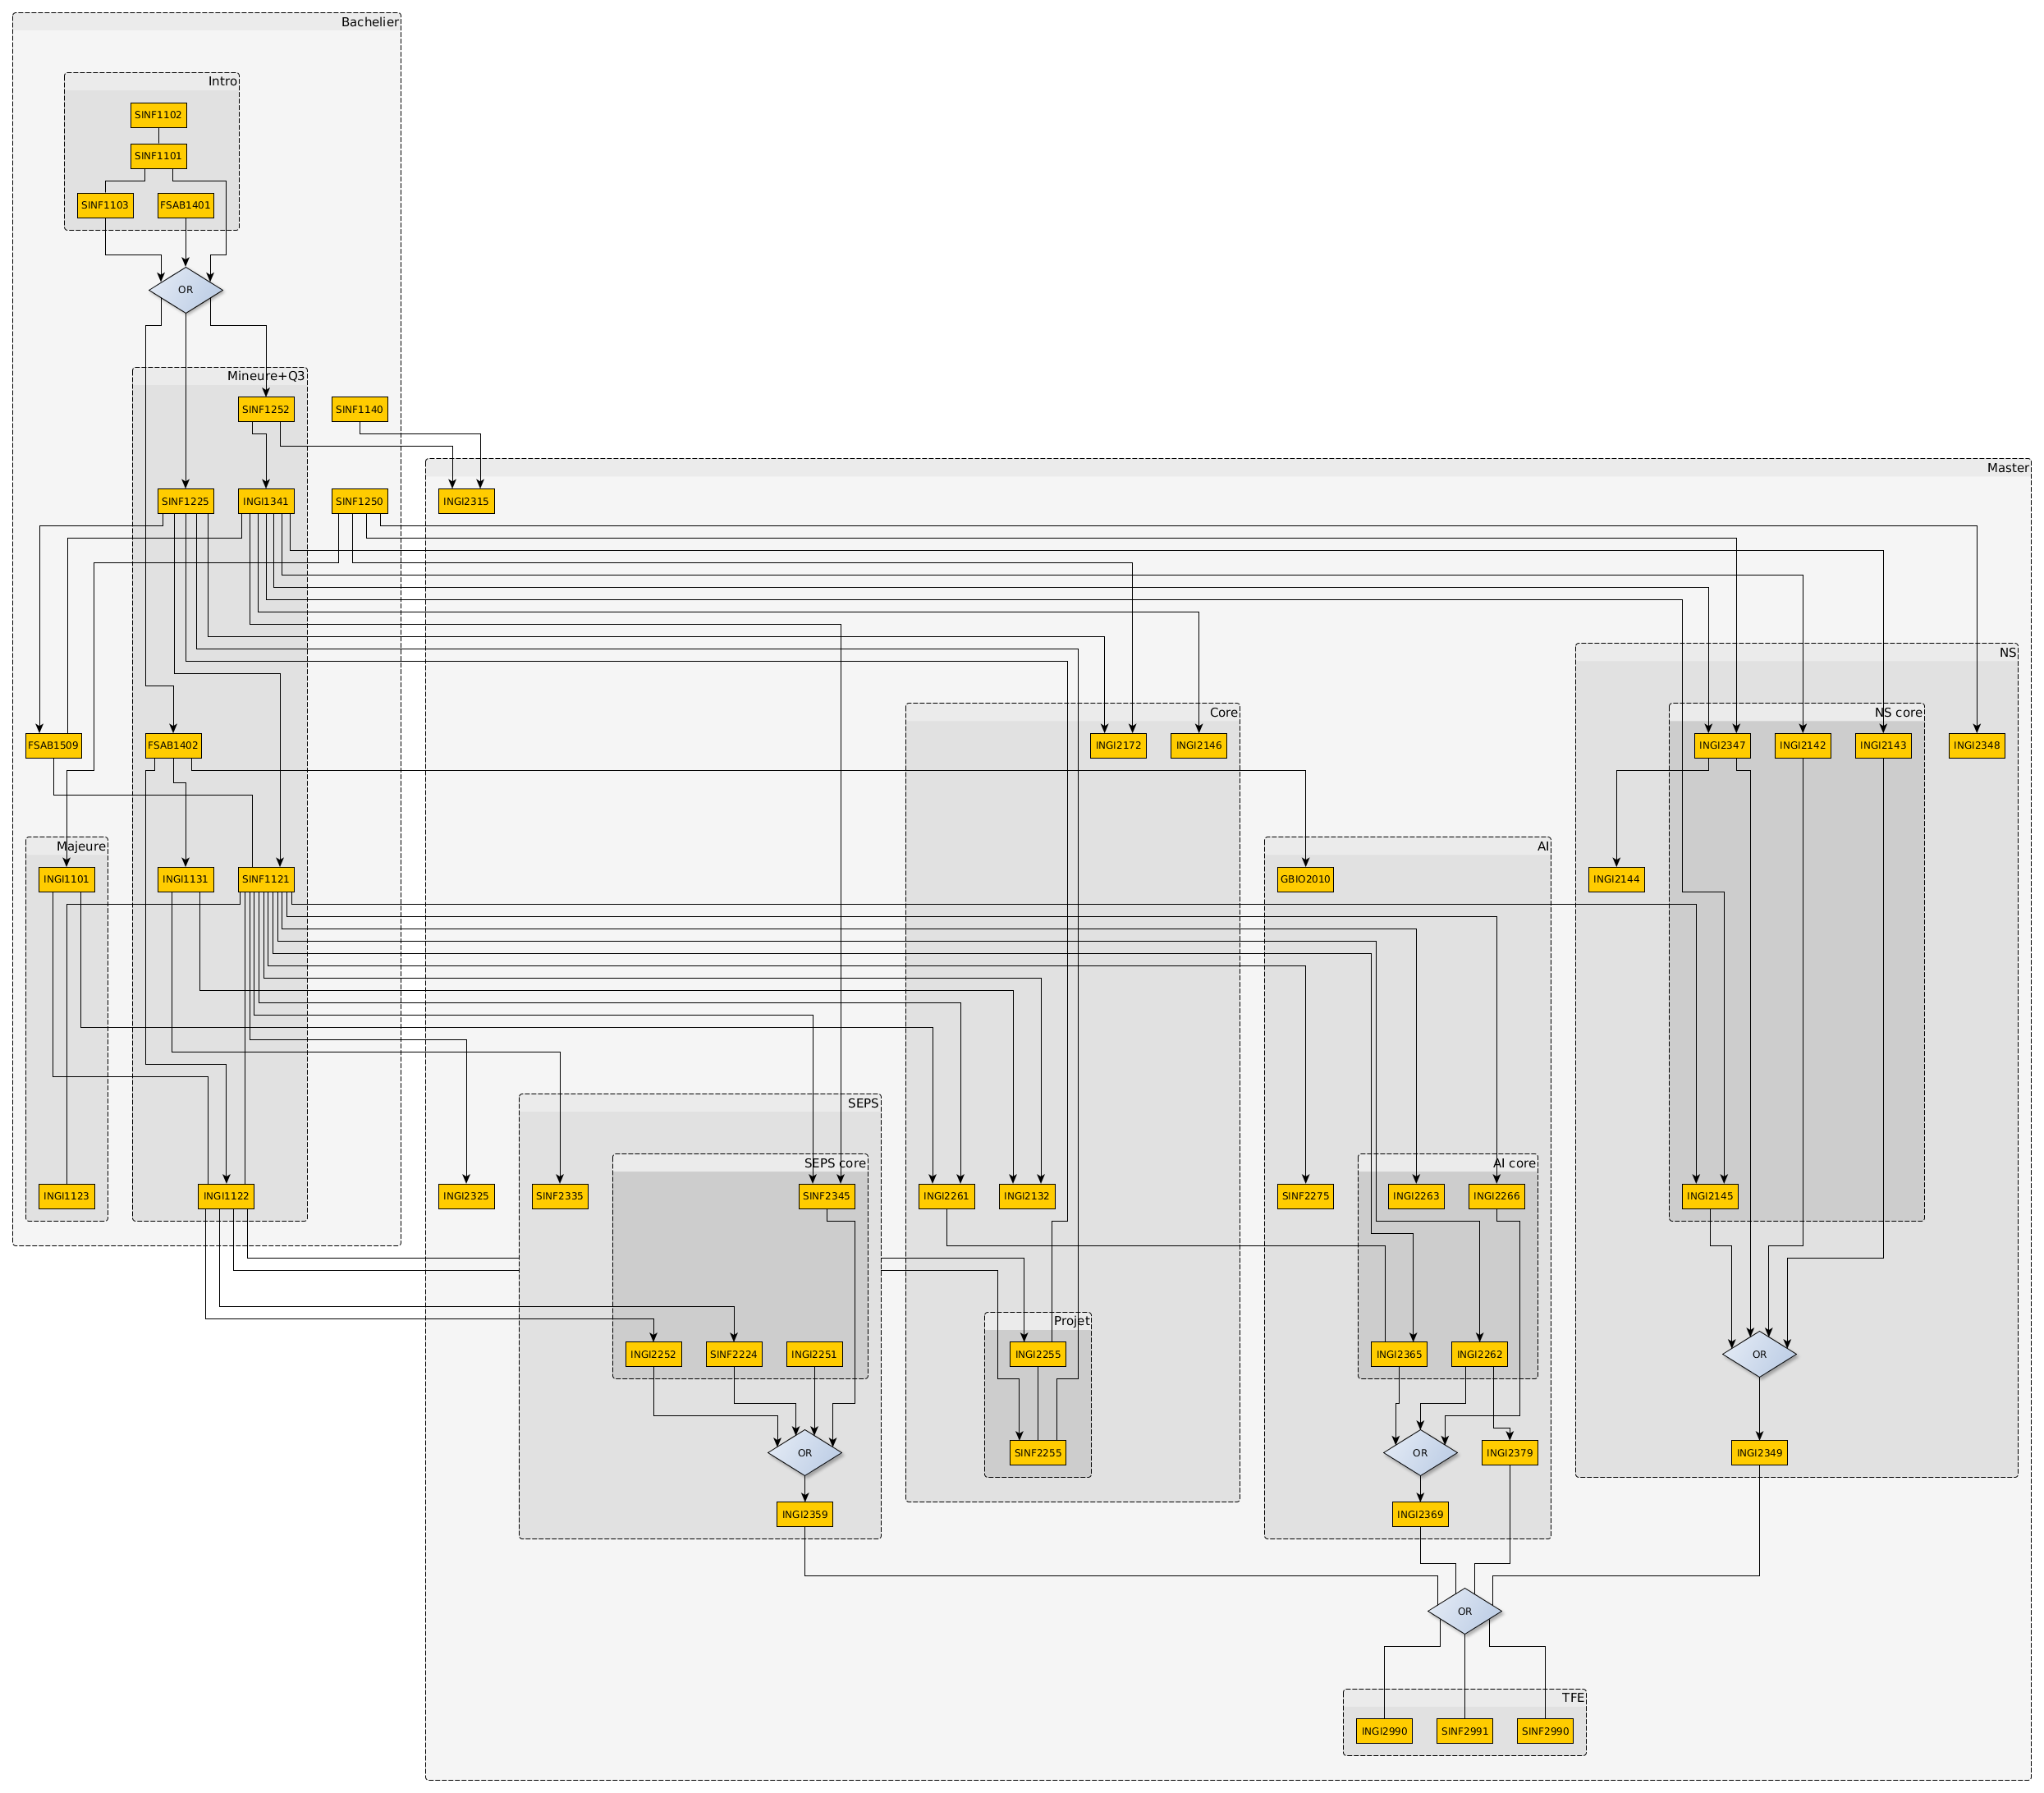
\includegraphics[width=\textwidth]{validation_init_graph}
\end{figure}

Après avoir importé le graphe, et ajouté les informations suivante dans le catalogue (via le formulaire Excel):
\begin{itemize}
\item tous les cours sont à 5 crédits, sauf les 3 mémoires (SINF2990 et INGI2990 à 28 crédits, SINF2991 à 18 crédits);
\item tous les cours sont alternés entre le premier et le second semestre, sauf les 3 mémoires qui sont marqué pour le second semestre;
\item on marque le module core (Master) et le module intro (Bachelier) comme obligatoire;
\item on ajoute un minimum de crédits à 20 et un maximum à 30 pour les trois options du programme de master;
\item on ajoute un minimum de crédits à 40 et un maximum à 80 pour le programme de bachelier;
\item on ajoute un minimum de crédits à 120 et un maximum à 150 pour le programme de master.
\end{itemize}   

Après avoir ajouté les informations, on marque le catalogue de cours comme principal, afin qu'il soit accessible aux étudiants.


\subsubsection{Configuration du programme de bachelier - Année 2006 à 2009}
Lorsque l'on configure le programme de bachelier, on remarque que le programme tel qu'il est conçu dans le graphe n'est pas \textit{validable} sur trois ans. En effet, il existe des \textbf{chaines de prérequis} dont la taille (en nombre de prérequis) est plus grande que trois, il faut donc étaler un programme sur plus de trois ans pour qu'il respecte les contraintes telles qu'elles sont présentées dans ce graphe, Une première amélioration à apporter à l'application est de détecter ces inconsistances lors de l'import du graphe dans l'application

Le programme ainsi configuré est validé par la commission. L'étudiant peut donc dès lors créer son programme de Master. 
\subsection{Premier scénario - Année académique 2009-2010}
L'étudiant va configurer son programme de master en:
\begin{itemize}
\item choisissant les cours qu'il va suivre durant l'année académique 2009-2010;

\item configurant l'année académique 2010-2011 pour s'assurer qu'il est possible de valider le programme dans lequel s'engage l'étudiant; cette année sera modifiable par la suite;

\item choisissant les modules optionnels qu'il compte suivre dans son programme.
\end{itemize}

Le programme de master comporte un module obligatoire (Core) et plusieurs modules optionnels (Génie logiciel, Intelligence artificiel et Réseau). L'étudiant décide de suivre l'option \textbf{Génie Logiciel} (SEPS sur le graphe). Ce module optionnel comporte un sous-module obligatoire (SEPS core)

Les cours suivis durant la premier année (2009-2010) sont les suivants:

\begin{table}[H]
\centering
\begin{tabular}{|c|c|c|}
\hline
\textbf{Cours} & \textbf{Crédits} & \textbf{Semestre}\\
\hline
INGI2315 & 5 & 1 \\
\hline
INGI2255 & 5 & 1 \\
\hline
INGI2172 & 5 & 1 \\
\hline
INGI2146 & 5 & 1 \\
\hline
SINF2345 & 5 & 1 \\
\hline
SINF2335 & 5 & 1 \\
\hline
INGI2325 & 5 & 2 \\
\hline
INGI2132 & 5 & 2 \\
\hline
INGI2261 & 5 & 2 \\
\hline
INGI2263 & 5 & 2 \\
\hline
SINF2275 & 5 & 2\\
\hline
\end{tabular}
\end{table}

Les cours que l'étudiant prévoit de suivre durant la seconde année (2010-2011) sont les suivants:

\begin{table}[H]
\centering
\begin{tabular}{|c|c|c|}
\hline
\textbf{Cours} & \textbf{Crédits} & \textbf{Semestre}\\
\hline
SINF2255 & 5 & 1\\
\hline
INGI2262 & 5 & 1\\
\hline
GBIO2010 & 5 & 1\\
\hline
INGI2251 & 5 & 1\\
\hline
SINF2224 & 5 & 1\\
\hline
SINF2290 &28 & 2 \\
\hline
INGI2379 & 5 & 2\\
\hline
INGI2252 & 5 & 2\\
\hline
INGI2359 & 5 & 2\\
\hline
\end{tabular}
\end{table}



L'étudiant décide de suivre l'option \textit{Software Engineering and Programming Systems (SEPS)}

Le programme de l'étudiant comporte une contrainte non respectée. En effet, il a décidé, durant la deuxième année, de suivre le cours INGI2379 (au second semestre)  et son prérequis INGI2262 (au premier semestre) durant la même année, ce qui enfreint la règle du prérequis. Cependant, il estime que, vu qu'il suit le cours INGI2262 au premier semestre et le cours INGI2379 au deuxième semestre cela ne pose pas de problème.

Il remplit donc la case justification de cette contrainte non respectée en expliquant la situation, avant d'envoyer sa demande de validation. 

L'étudiant va ensuite négocier la validation de son programme avec la commission de programme, puis celle-ci va valider son programme après quelques discussions. 

La commission de programme reçoit la demande de validation, regarde son programme et voit que:
\begin{itemize}
\item le programme de master comporte assez de crédits (123);
\item l'ensemble des modules obligatoires est présent;
\item une option est présente;
\item un prérequis est enfreint.
\end{itemize}

La commission de programme regarde la justification de l'étudiant (il est obligé d'en remplir une si son programme ne respecte pas toutes les contraintes). Elle regarde la justification, et refuse la demande de validation en demandant à l'étudiant de choisir un autre cours (ou bien de suivre le prérequis durant l'année précédente).

Ici, une première amélioration pourrait être apportée à l'application. Il faudrait permettre à la commission de maquer chaque justification de contrainte non respectée comme acceptée ou refusée. L'étudiant pourrait ainsi voir plus clairement les parties qui ne sont pas valides dans sa demande de validation.  

L'étudiant retourne sur son programme, voit qu'il a un nouveau message en attente. Il choisi un autre cours (LINGI2143) et renvoie sa demande de validation qui est ensuite validée par la commission.

Ici, une seconde amélioration pourrait être apportée à l'application. L'étudiant n'est pas clairement averti que sa demande a été refusée. Tout ce qu'il voit, c'est que son programme n'est toujours pas validé et qu'il a la possibilité de renvoyer une demande de validation. 

\subsection{Second scénario - Année académique 2010-2011}
L'année académique suivante, l'étudiant a réussi son année. La commission marque son année comme réussie. Cependant, la commission de programme ajoute une nouvelle version du catalogue de cours qui modifie le programme de master.

L'application n'a aucun problème pour récupérer les contraintes des anciens programmes de cours. Par contre, si l'on renomme des cours, elle ne pourra pas récupérer les anciennes instances des cours (la recherche se faisant sur le nom du cours). De plus, si ces cours on déjà été suivis par des étudiants, et qu'ils jouent le rôle de prérequis ou de corequis pour des cours présents dans des années qui ne sont pas encore validées, les étudiants concernés auront à justifier ces dépendances manquantes dans leur programme. 

C'est pourquoi, la modification se portera essentiellement sur le nom de cours qui sont des dépendances pour des cours choisis dans la seconde année académique de l'étudiant.


On déclenchera ainsi un processus de négociation dans lequel l'étudiant expliquera qu'il a déjà suivi les anciennes versions des cours. De plus, l'application, pour le moment ne gère pas la récupération des anciens modules choisis. L'étudiant doit à nouveau choisir le module correspondant. 

La modification apportée au catalogue sont les suivantes:
\begin{itemize}
\item renommage du cours \textit{INGI2252} en \textit{INGI2252BIS};
\item renommage du cours \textit{SINF2224} en \textit{SINF2224BIS};
\item renommage du cours \textit{INGI2251} en \textit{INGI2251BIS};
\item renommage du cours \textit{SINF2345} en \textit{SINF2345BIS}.
\end{itemize}

La commission crée un nouveau catalogue de cours comportant ces modifications, avec le même nom que le précédent, mais en changeant l'année académique qui l'identifie. 

Lorsqu'une version plus récente du catalogue de cours utilisé par l'étudiant est importé dans l'application, il est proposé à celui-ci de mettre à jour son programme. L'étudiant va donc, au début de l'année académique 2010-2011 mettre à jour son programme de cours, avant de configurer sa dernière année et de renvoyer son programme à la validation.

L'étudiant est invité, lorsqu'il se rend sur la page de configuration de son programme de cours, à migrer le programme de cours qu'il suit vers sa nouvelle version.

L'étudiant se retrouve donc avec des dépendances manquantes liées au cours qui ont changé de nom. 

L'étudiant n'a donc qu'à expliquer qu'il a bien suivit ces cours. La commission peut quant à elle facilement vérifier de son coté que les cours ont bien été suivit lors des années précédentes. Elle n'a plus ensuite qu'à valider le programme de l'étudiant. 


\section{Conclusion}

Les scénarios présentés sont assez complets que pour illustrer la plupart des fonctionnalités de l'application. Ils ont permi d'identifier certaines fonctionnalités qui manquent encore à l'application à savoir:
\begin{itemize}
\item afficher plus clairement à l'étudiant que sa demande de validation a été refusée;
\item permettre à la commission de programme d'accepter ou de refuser chaque message de justification de l'étudiant pour qu'il puisse savoir quelles justifications ne sont pas suffisantes.
\end{itemize}

Le chapitre suivant présentera des pistes de travaux futurs. 